\chapter{Туршилт, үр дүн}
\label{Chapter4}

\section{Системийн ажиллагааны тест}
\subsection{Insomnia тест}
Системийн API endpoint-уудыг шалгахын тулд insomnia ашигласан.
\begin{figure}[htbp]
    \centering
    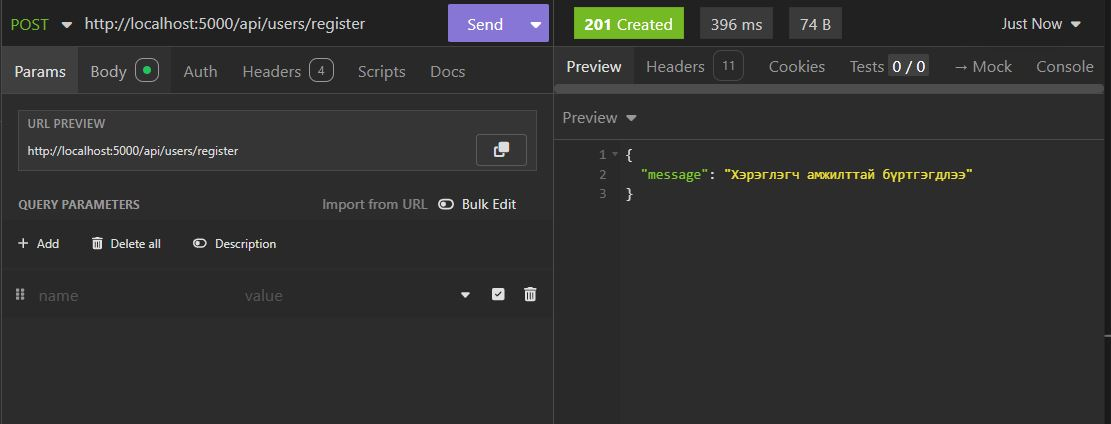
\includegraphics[width=0.9\textwidth]{Diagrams/registerinso}
    \caption{Бүртгүүлэх api}
    \label{fig:activity1}
\end{figure}
\begin{figure}[htbp]
    \centering
    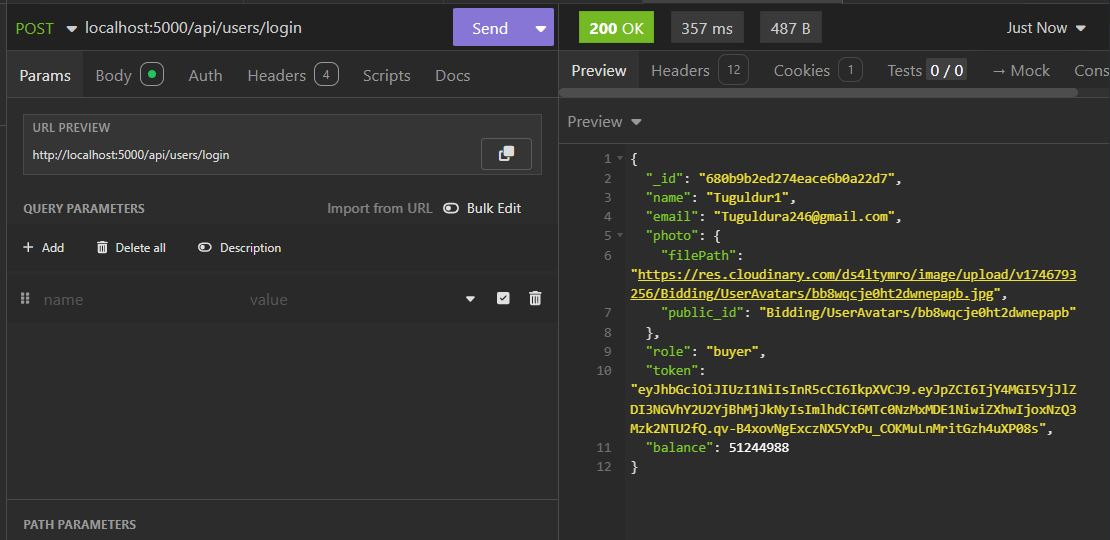
\includegraphics[width=0.9\textwidth]{Diagrams/logininso}
    \caption{Нэвтрэх api}
    \label{fig:activity1}
\end{figure}
\begin{figure}[htbp]
    \centering
    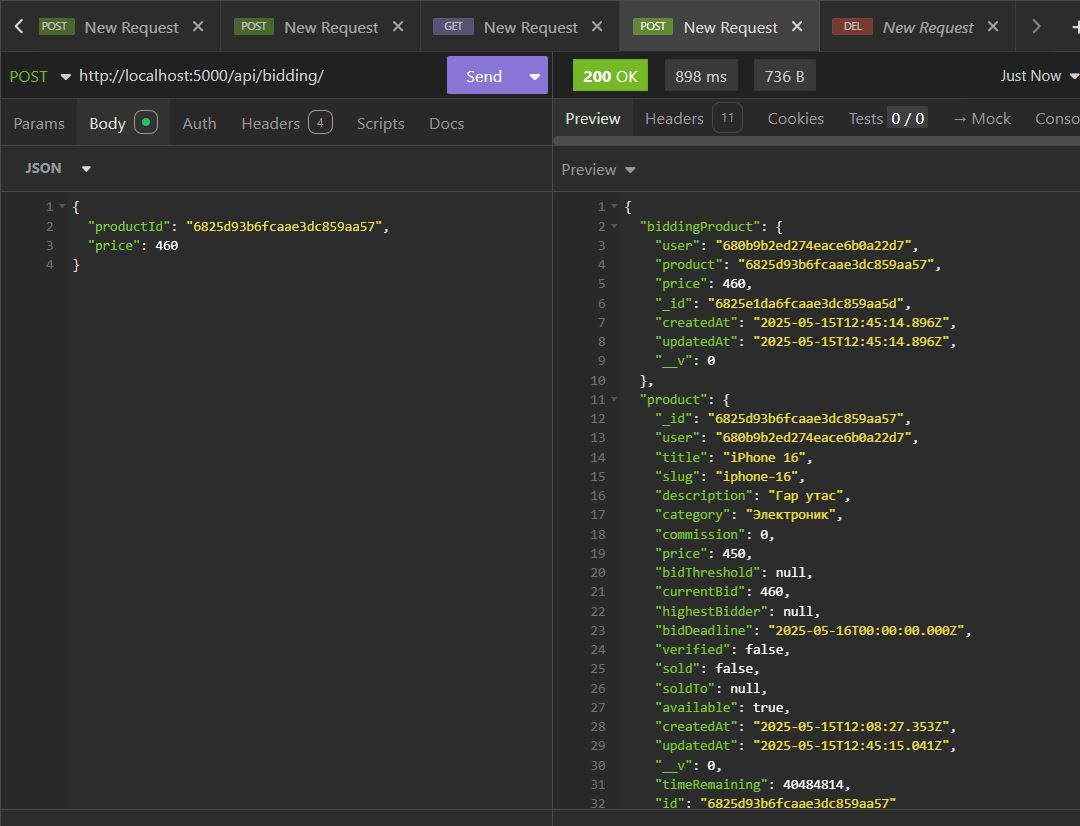
\includegraphics[width=0.7\textwidth]{Diagrams/biddinginso}
    \caption{Үнэ санал болгох api}
    \label{fig:activity1}
\end{figure}
\begin{figure}[htbp]
    \centering
    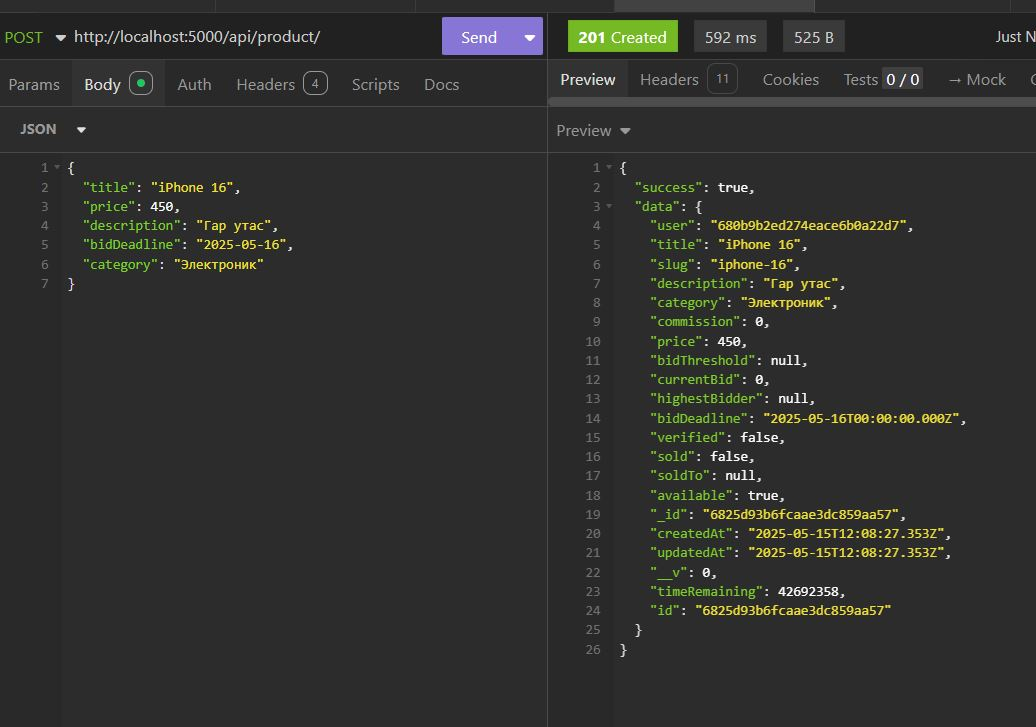
\includegraphics[width=0.7\textwidth]{Diagrams/postproduct}
    \caption{Бараа нэмэх api}
    \label{fig:activity1}
\end{figure}
\newline
Бүртгүүлэх, нэвтрэх, үнэ санал болгох, бараа нэмэх гэх мэт үйлдлүүдийг хийх API-уудыг insomnia ашиглаж ажиллагааг шалгаж үзэв. 
\newpage
\subsection{Unit test}
Системийн үндсэн гол функцуудэд jest Javascript ашиглан логик үйлдлүүдэд тус бүр test хийж шалгасан.Жишээлбэл, дуудлага худалдаанд үнэ өгөх хэрэглэгч бүртгэх нэвтрэх гэх мэт үйлдлүүдэд mock мэдээллээр хүсэлт илгээж хариу тус бүрийг шалгасан.
\newline \textbf{BiddingController test} 
\begin{figure}[htbp]
    \centering
    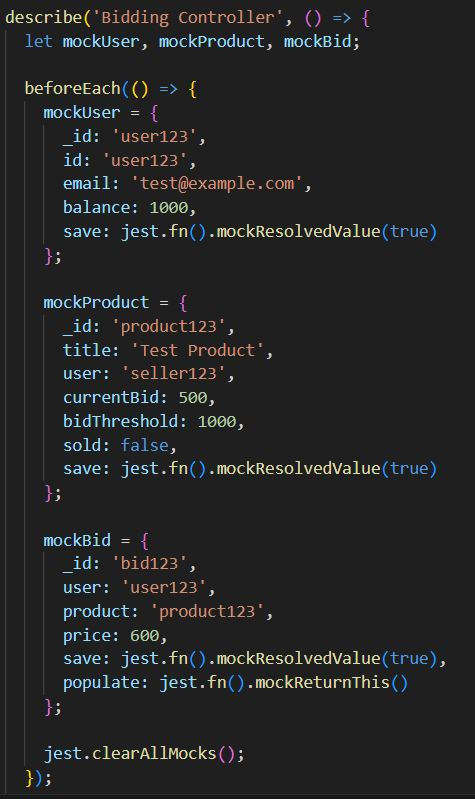
\includegraphics[width=0.5\textwidth]{Diagrams/testbidding}
    \caption{Үнэ өгөх тест 1}
    \label{fig:activity1}
\end{figure}
\begin{figure}[htbp]
    \centering
    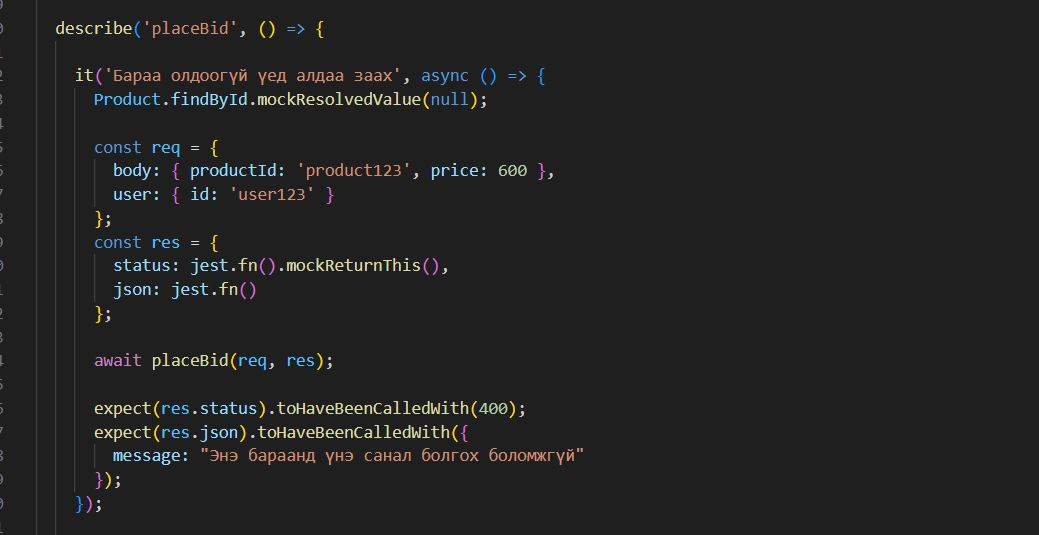
\includegraphics[scale=0.6]{Diagrams/bidtest}
    \caption{Үнэ өгөх тест 2}
    \label{fig:activity1}
\end{figure}
\begin{figure}[htbp]
    \centering
    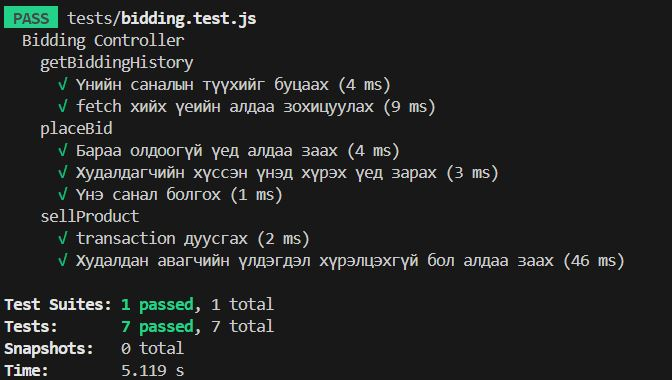
\includegraphics[width=0.7\textwidth]{Diagrams/biddingres}
    \caption{Үнэ өгөх тест хариу}
    \label{fig:activity1}
\end{figure}

\clearpage
\textbf{UserController test}
\begin{figure}[htbp]
    \centering
    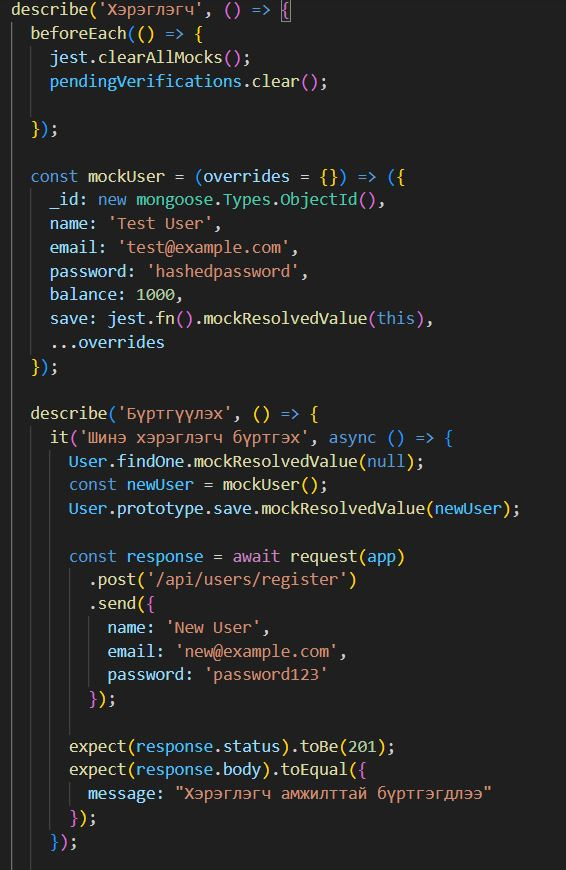
\includegraphics[width=0.7\textwidth]{Diagrams/testuser}
    \caption{Бүртгүүлэх функц}
    \label{fig:activity1}
\end{figure}
\begin{figure}[htbp]
    \centering
    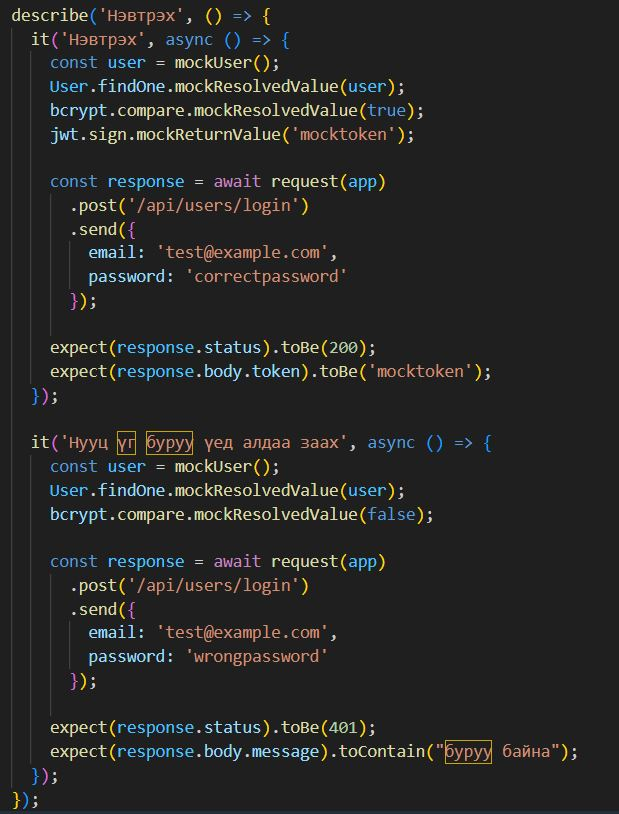
\includegraphics[width=0.5\textwidth]{Diagrams/testuser1}
    \caption{Нэвтрэх функц}
    \label{fig:activity1}
\end{figure}
\begin{figure}[htbp]
    \centering
    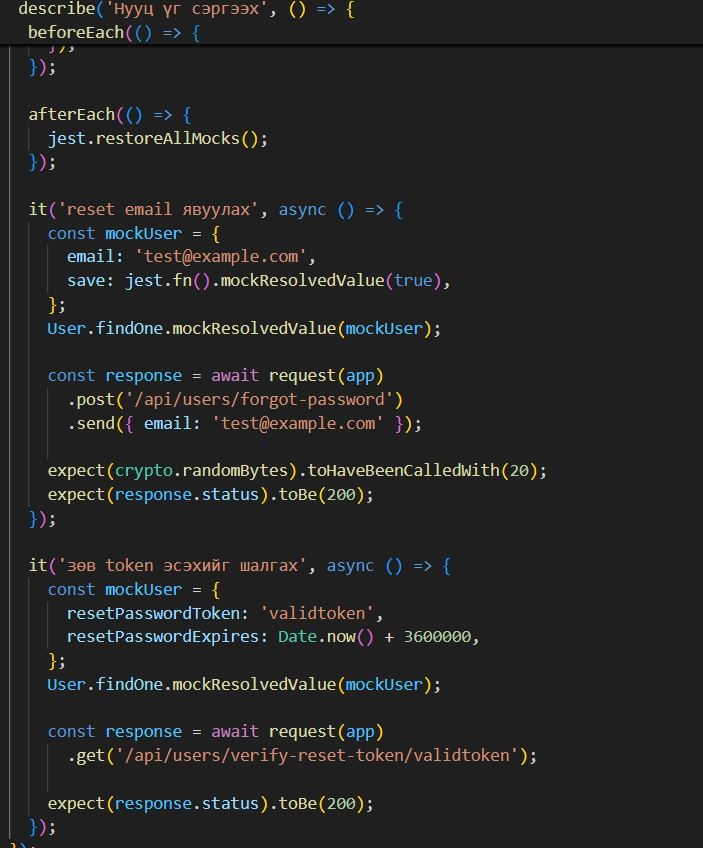
\includegraphics[width=0.5\textwidth]{Diagrams/testuser3}
    \caption{Нууц үг сэргээх функц}
    \label{fig:activity1}
\end{figure}


\begin{figure}[htbp]
    \centering
    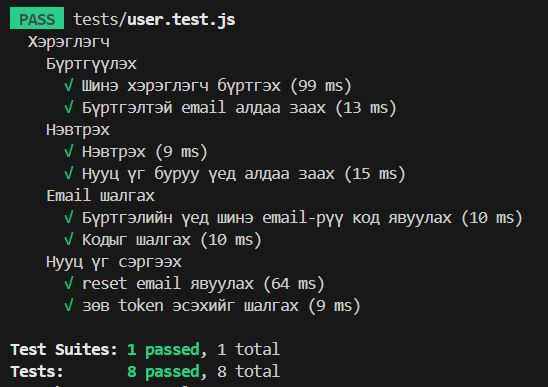
\includegraphics[width=0.6\textwidth]{Diagrams/userresult}
    \caption{Хэрэглэгчийн тестийн хариу}
    \label{fig:activity1}
\end{figure}
\newpage
\textbf{ProductController test}
\begin{figure}[htbp]
    \centering
    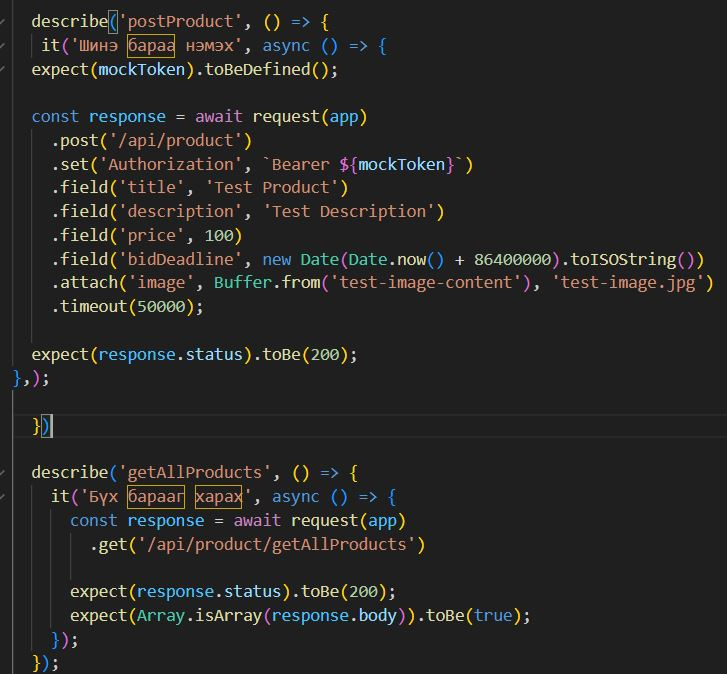
\includegraphics[width=0.7\textwidth]{Diagrams/testpro}
    \caption{Барааг нэмэх, Бараа үзэх функц}
    \label{fig:activity1}
\end{figure}
\begin{figure}[htbp]
    \centering
    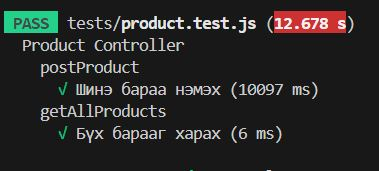
\includegraphics[width=0.7\textwidth]{Diagrams/productresult}
    \caption{Барааны тестийн хариу}
    \label{fig:activity1}
\end{figure}
\newline
Манай онлайн дуудлага худалдааны системд юнит тест хэрэглэх гол шалтгаанууд:

\begin{itemize}
\item Функц/модуль бүрийн зөв ажиллахыг баталгаажуулах
\item Алдааг эрт олно
\item Тест нь код хэрхэн ажиллах ёстойг харуулна
\end{itemize}
\subsection{Integration test}
Манай онлайн дуудлага худалдааны системийн үндсэн функцүүдийн хоорондын уялдаа холбоог интеграцийн тестээр шалгасан. Энэ нь:

\begin{itemize}
\item Модуль хоорондын интерфейс зөв ажиллах
\item Өгөгдлийн урсгал бүрэн бүтэн байх
\item Алдааны тохиолдолд зохих мессеж буцаах
\end{itemize}
\begin{figure}[htbp]
    \centering
    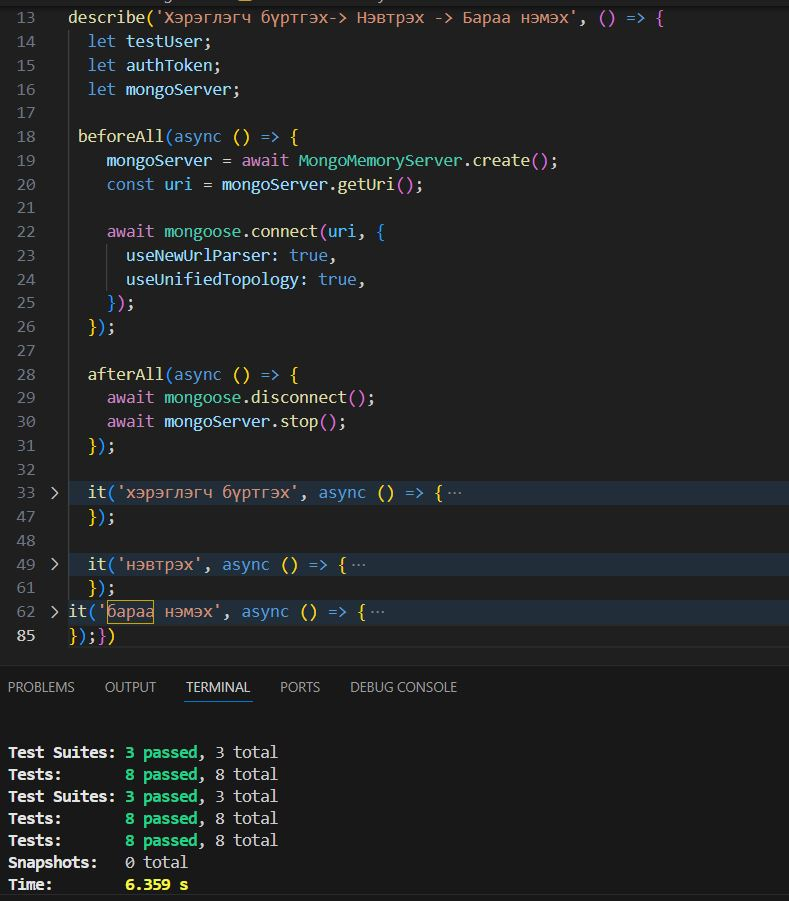
\includegraphics[width=0.7\textwidth]{Diagrams/addproductinteg}
    \caption{Бараа нэмэх функийн интеграци}
    \label{fig:activity1}
\end{figure}
\begin{figure}[htbp]
    \centering
    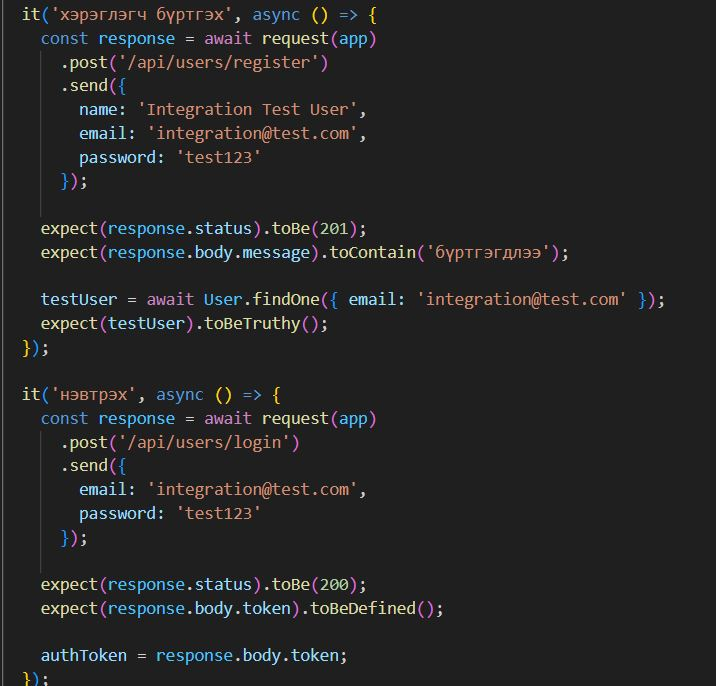
\includegraphics[width=0.7\textwidth]{Diagrams/integ}
    \caption{Хэрэглэгч бүртгүүлэх нэвтрэх функууд }
    \label{fig:activity1}
\end{figure}
\begin{figure}[htbp]
    \centering
    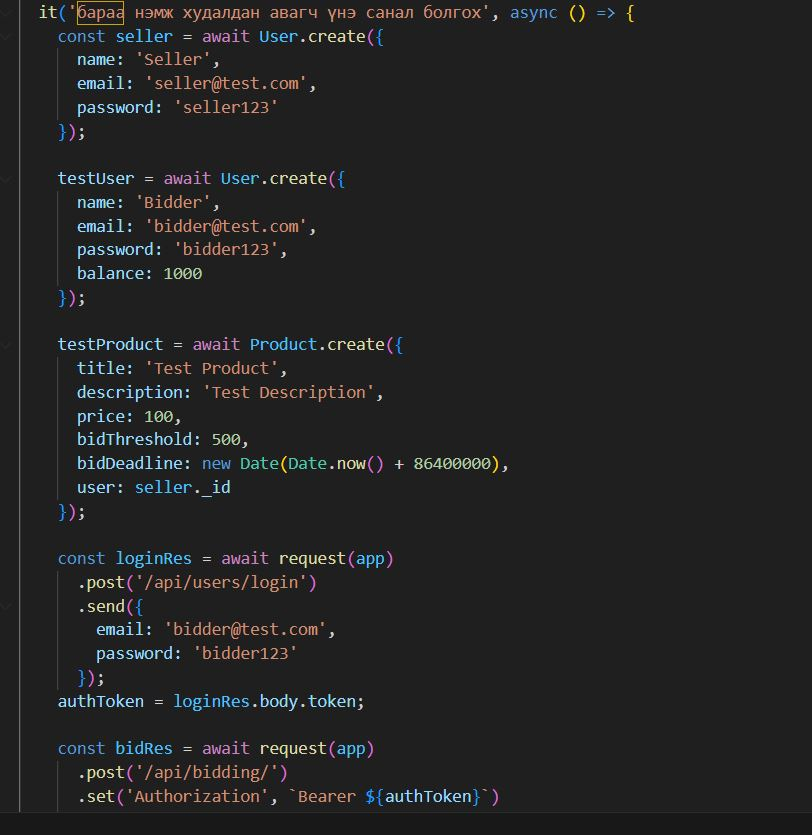
\includegraphics[width=0.7\textwidth]{Diagrams/placebidint}
    \caption{Үнэ өгөх функцийн интеграци 1}
    \label{fig:activity1}
\end{figure}
\begin{figure}[htbp]
    \centering
    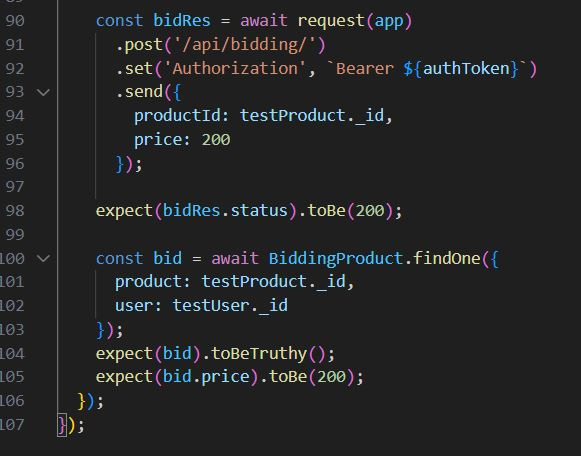
\includegraphics[width=0.7\textwidth]{Diagrams/placebidint2}
    \caption{Үнэ өгөх функцийн интеграци 2}
    \label{fig:activity1}
\end{figure}
\clearpage